
{\bf\large Names:}


\subsection*{Scale Dependent Parametrizations}

Consider a steady flow of 10 cm s$^{-1}$ over a flat bottom in a turbulent ocean.  We will neglect impacts of stratification and rotation.  In a large scale ocean model we would parametrize the drag of the bottom using an nonlinear, quadratic drag law of the form:

\begin{equation}
\tau = C_D \rho u^2
\label{eq:drag}
\end{equation}
where $\tau$ is bottom drag or stress, $\rho \approx 1000$ kg m$^{-3}$ is the density of water, $u$ is the flow speed above the bottom and $C_D$ is the drag coefficient.  The drag coefficient is a bit of a fudge factor and depends on your problem.  Here we will use 0.01.  In SalishSeaCast I tune it to get the tides accurate.

\begin{question}
What is the drag? \\
$\tau = $\\[24pt]
\end{question}

Let's look a little closer, below is a grid diagram
(Figure~\ref{plt:grid}).  Given the flow of 10 cm s$^{^-1}$ at the
lowest grid cell $u_1$, the drag on that velocity is the value given above.

\begin{figure}[h]
\resizebox{3in}{!}{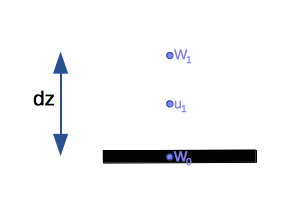
\includegraphics{grid.png}}
\caption{\protect\it{Typical grid near the bottom. $w$ is the vertical
    velocity, the black line is the bottom. No flow through the bottom
    implies $w_0 = 0$.} Lowest horizontal velocity grid point $u_1$ is
  $dz/2$ from the bottom.}
\label{plt:grid}
\end{figure}

\clearpage

In the ``real world'' we would expect a log layer profile (Figure~\ref{plt:loglayer}):

\begin{equation}
u = \max \left[ \frac {u_*}{\kappa} \log \left( \frac z z_* \right), U \right]
\end{equation}
where $u_* = (\tau/\rho)^{1/2}$ is the friction velocity, $\kappa =
0.41$ is von Karman's constant, $z$ is height above the bottom, $z_*$
is the roughness length, here 20 cm, and $U$ is the free stream (above boundary layer) velocity.

\begin{figure}[ht]
\resizebox{5.5in}{!}{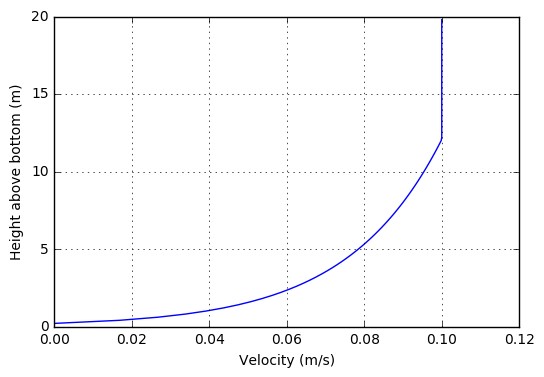
\includegraphics{loglayer.png}}
\caption{\protect\it{Log layer velocity profile.}}
\label{plt:loglayer}
\end{figure}

To match the log-layer to the bottom stress parametrization above we
find that 
\begin{equation}
u_* = \frac U {C_D^{1/2}}
\end{equation}

Let's assume that the model velocity at each grid point is exactly the log
layer value at the appropriate height above the bottom.  That is, you can
find $u_1$ from Figure~\ref{plt:loglayer} by reading off the graph the
value at $dz/2$.

For a large scale model a  typical bottom layer box thickness, $dz =
30$~m.  In coastal models we usually have better resolution.  What
happens if we use the parametrization (\ref{eq:drag}) but have better resolution?

\clearpage

\begin{question}
What is the drag using the quadratic drag law  (\ref{eq:drag}) for the
flow shown in Figure~\ref{plt:loglayer} for bottom grid resolutions of
$dz = $10, 5 and 2 m?\\
With $dz=10$m , $\tau  = $\\[24pt]
With $dz=5$m , $\tau  = $\\[24pt]
With $dz=2$m , $\tau  = $\\[12pt]
\end{question}

\begin{question}
Should the drag change in this way? Why or why not?
\end{question}

\vspace{1in}

\begin{question}
Noting that our bottom grid cells are not always the same size, in
shallower water they are often smaller, how should we parametrize the
bottom drag?\\[24pt]
\end{question}